\chapter{Кодирование}

\section{Хранение информации}

\subsection{Деревья поиска}

\subsubsection{AVL дерево}

\begin{definition}
	Высота дерева -- длина максимального пути от корня до листа
\end{definition}

\begin{definition}
	Вершина сбалансирована, если высоты её левого и правого поддерева оличаются не больше, чем на 1
\end{definition}

\begin{definition}
	Дерево сбалансировано, если все вершины сбалансированы
\end{definition}

\begin{algorithm}
    \hfill
    \begin{enumerate}
    	\item Добавим вершину $d$.
        \item Проверяем вершины на пути от $d$ к корню на сбалансированность.
        \item Обозначим через $a$ первую на этом пути несбалансированную вершину. $b$ и $c$ -- её потомки
        \item Балансируем дерево (``поднимаем'' несбалансированную вершину) (тут должны быть картинки)
    \end{enumerate}

\end{algorithm}

\subsubsection{Некая структура}

Выбирается $n$ -- диапазон ключей. Есть некий массив от 0 до $n-1$. В каждом элементе ссылка на набор записей. Мы придумали, как ключ переводить в $i \in 0:n-1$ Чтобы найти запись с нужным ключом, находим $i$, а потом просматриваем список. Чтобы добавить запись, вычисляем $i$ и добавляем в набор по его правилам (вдруг мы хотим, чтобы набор был отсортирован). Какую бы мы ни взяли хеш-функцию, последним действием всегда будет взятие статка по модулю $n$. Хорошая хеш-функция перемешивает максимально равномерно

\subsubsection{B-деревья}

\begin{definition}
    \hfill
    \begin{itemize}
    	\item Все листья на одном уровне
        \item Записи хранятся в листьях
        \item Число записей индекса -- $2d - 1 \ge 3$
        \item Число записей в блоке -- $2e - 1 \ge 3$
    \end{itemize}
    $e$ и $d$ мы выбираем. Можно иметь пустые места, но записей должно быть как минимум $d$ (или $e$)
\end{definition}


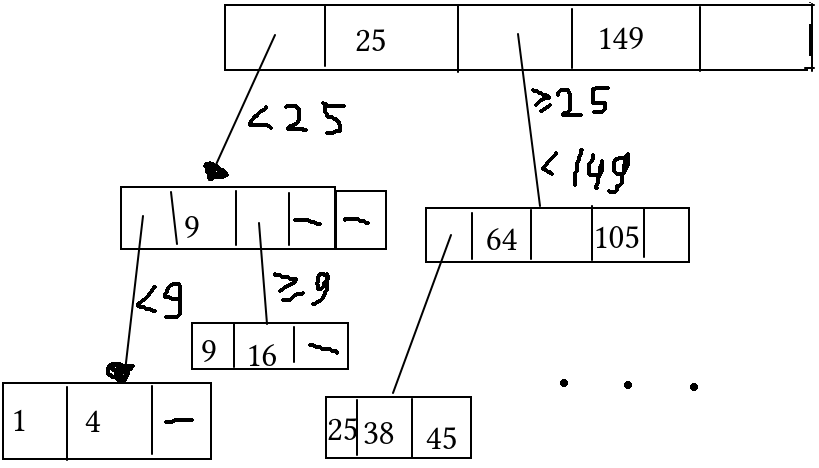
\includegraphics[scale=0.6]{1}

Нужно добавить 32:

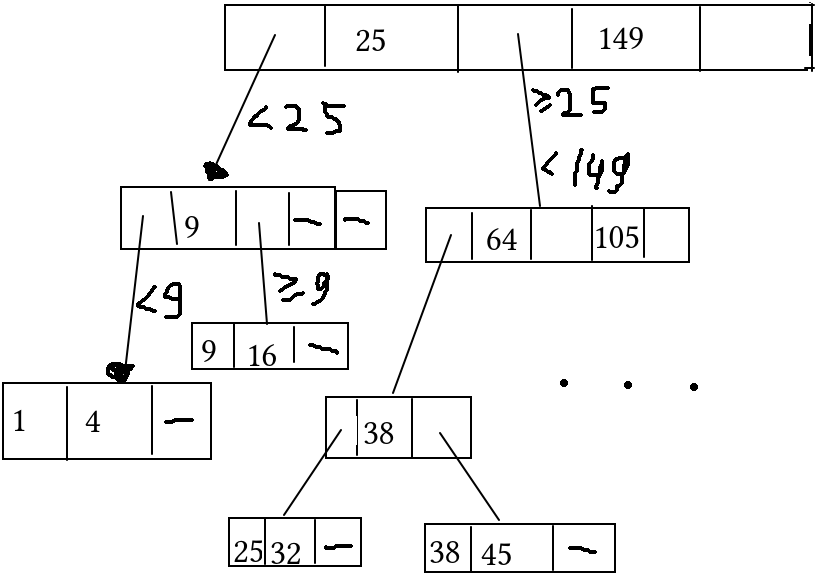
\includegraphics[scale=0.6]{2}
\\
Дальше ещё картинки, но там нихуя не понятно \\
Удаление: если запись первая в блоке, возможно, придётся поменять индекс в родиетеле. Если после удаления записей стало меньше, чем нужно, то ``пристраиваем'' её куда-нибудь (с заменой индекса родителя. Возможно, придётся перестаивать дальше)
